\chapter{Implementation}
Each unit is described by the following procedure:
\begin{itemize}
\item Overall design and block description
\item Individual block breakdown
\item Block construction
\end{itemize}
This procedure is meant to ease readability and help give an overview of the entire system implementation.
\section{CDU}

\section{Sensor Node}
The sensor node responsibility is, as described in the previous documents, to capture a temperature and support the custom powerline communication protocol. Below is described in detail how each block in the sensor node is implemented and designed.

\subsection{Overall design}
Below is shown a figure of the overall sensor node design.
\begin{figure}
\centering
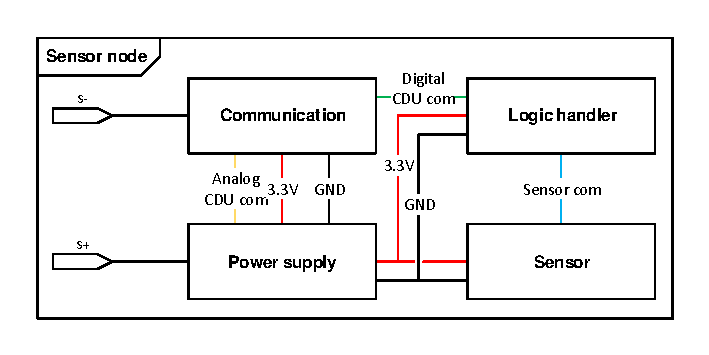
\includegraphics[width=.9\textwidth]{billeder/sn_overall_design}
\caption{Sensor node overall design}
\end{figure}

\subsubsection{Block description}
\textbf{Power supply:}\\
The power supply is creates a steady 3.3V supply to the system from the powerline communication bus.\\

\textbf{Communication:}\\
The communication block convertes the analog communication signal from the CDU to a digital stream of data and clock to the system and the digital communication from the logic handler to an analog signal on the bus to the CDU.\\

\textbf{Logic handler:}\\
The logic handler 

\subsection{Power supply}
The power supply block is responsible for power to the entire sensor. This involves making 3.3V to the system in the sensor node and thereby making a reference voltage as ground to the system. Below in figure \ref{fig:SN_PS_FIGURE} is shown the interface to the power supply.
\begin{figure}[H]
\centering
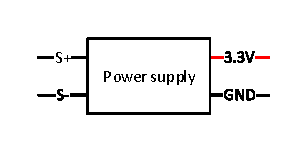
\includegraphics[width=.5\textwidth]{billeder/sn_powersupply_figure}
\caption{Sensor node power supply block}
\label{fig:SN_PS_FIGURE}
\end{figure} 
The goal is to create a steady 3.3V power to the components on the sensor node. The bus is specified as a line where all sensor nodes are placed in series. Therefore each sensor node has to create its own reference ground from the line. The line is a constant current modulated with communication.\\
The S+ and S- signals are from the powerline bus where S+ is connected to the previous sensor or the CDU B+ pin. The S- is connected to the next sensor or the CDU B- pin.\\

Below in figure xx is shown the implementation of the Power supply block.




\subsection{Communication}




\subsection{Logic handler}

\subsection{Sensor}